\documentclass[a4paper,11pt,notitlepage]{report}

% Language and encoding
\usepackage[utf8]{inputenc}
\usepackage[T1]{fontenc}
\usepackage[english]{babel}
\usepackage{lmodern}         
\renewcommand{\rmdefault}{bch}

% Page layout
\usepackage{geometry}
\geometry{a4paper, margin=1in}

% Packages for styling
\usepackage{amsmath, amssymb} % For mathematical formulas
\usepackage{booktabs}         % For professional tables
\usepackage[hypertexnames=false]{hyperref}         % For clickable links
\usepackage{setspace}         % For line spacing
\usepackage{titlesec}         % For section formatting
\usepackage{graphicx}         % For images
\usepackage{float}            % For figure placement

\setstretch{1.2} % Adjust line spacing

% Hyperlinking
\hypersetup{
    colorlinks=true,
    linkcolor=black,
    filecolor=black,
    urlcolor=black, 
    citecolor=blue
}

\onehalfspacing

% Title Page Info
\title{
    \textbf{\Huge NeuroShot: Final Report} \\
    \Large Dynamic Trajectory Optimization for Moving Targets using DRL \\
    \vspace{0.5cm}
    \normalsize DA 346: Deep Reinforcement Learning
}
\author{Team Insight Engineers}
\date{\today}

\begin{document}
\fontsize{11}{15}\selectfont

\makeatletter
\renewcommand*{\theHfigure}{\arabic{figure}}
\renewcommand*{\theHtable}{\arabic{table}}
\makeatother

\maketitle

\begin{center}
    \begin{tabular*}{0.85\textwidth}{@{\extracolsep{\fill}}ccc}
        \multicolumn{3}{c}{\large Project by} \\ [0.5ex] 
        \midrule 
        \textbf{Niladri Ghosh} & \textbf{Raihan Uddin} & \textbf{Sayan Das} \\
        B2430100 & B2430070 & B2430035 \\
    \end{tabular*}
\end{center}
\hrule
\vspace{1cm}

\section*{\centering Abstract}
\addcontentsline{toc}{section}{Abstract}
This report presents a two-part final project for DA 346: Deep Reinforcement Learning. In Part 1, we conduct a comparative study of three widely used deep reinforcement learning algorithms: Proximal Policy Optimization (PPO), Advantage Actor--Critic (A2C), and Soft Actor--Critic (SAC) on the Gymnasium continuous-control benchmark LunarLanderContinuous\allowbreak -v3. We formalize the benchmark as a Markov Decision Process (MDP), document architectures and hyperparameters, and report learning dynamics with mean and variance across training seeds. In Part 2, we design a custom environment, NeuroShot-v1, modeling anticipatory ballistic interception of a moving oscillatory target under stochastic wind. We specify the custom MDP, justify algorithm choice, and evaluate training behavior and final policy performance under randomized conditions. Across both parts, we emphasize mathematical correctness, experimental rigor, and a critical theory--practice synthesis.

\section*{\centering Overview}
\addcontentsline{toc}{section}{Overview}
The project consists of two connected components consolidated in a single report. Part 1 focuses on benchmarking algorithmic behavior under a fixed interaction budget and controlled experimental conditions. Part 2 focuses on environment design, reward shaping trade-offs, and agent training in a custom decision-driven setting. Unless stated otherwise, all experiments were executed on a CPU-only workstation running Windows 11 (20 logical CPU cores) with a PyTorch CPU backend~\cite{pytorch} and without GPU acceleration.

\tableofcontents
\newpage

\chapter{Part 1: Comparative Study of Deep RL Algorithms}

\section{1.\ Problem Selection}
For the comparative study of canonical deep reinforcement learning methods, we selected the continuous-control benchmark \textbf{LunarLanderContinuous-v3} from Gymnasium~\cite{gymnasium}. This task is widely used to evaluate learning in a moderately high-dimensional continuous action space under stochastic initial conditions and non-linear contact dynamics.

\subsection{Rationale and Non-triviality}
The task is non-trivial for at least three reasons.
\begin{itemize}
    \item \textbf{Control coupling and stability:} The agent must simultaneously regulate translational motion and attitude. Small deviations in angle can induce large changes in horizontal drift, and contact events with the ground introduce discontinuities in the dynamics.
    \item \textbf{Sample-efficiency requirements:} Reward shaping is present, but meaningful improvements require coordinated sequences of thrust decisions. Algorithms that discard data after each update (on-policy) may require substantially more environment interaction than algorithms that reuse experience (off-policy).
    \item \textbf{Convergence difficulty under exploration:} The agent must balance exploration (to discover stabilizing maneuvers) with conservative refinement (to avoid destabilizing updates). This amplifies sensitivity to update magnitude and value-function approximation error.
\end{itemize}

\section{2.\ Algorithms Studied}
We studied three algorithms spanning key design axes: \textbf{PPO} (on-policy, trust-region inspired)\allowbreak~\cite{schulman2017ppo}, \textbf{A2C} (on-policy, actor--critic with $n$-step returns)\allowbreak~\cite{mnih2016a3c}, and \textbf{SAC} (off-policy, maximum-entropy)\allowbreak~\cite{haarnoja2018sac}.

\subsection{Proximal Policy Optimization (PPO)}
Let $\pi_\theta(a\mid s)$ denote a stochastic policy and let $\hat{A}_t$ be an estimator of the advantage $A^{\pi}(s_t,a_t)=Q^{\pi}(s_t,a_t)-V^{\pi}(s_t)$. PPO maximizes a clipped surrogate objective that constrains policy updates in terms of the probability ratio
\[
r_t(\theta)=\frac{\pi_\theta(a_t\mid s_t)}{\pi_{\theta_{\mathrm{old}}}(a_t\mid s_t)}.
\]
The clipped objective is
\[
\mathcal{L}_{\mathrm{CLIP}}(\theta)=\hat{\mathbb{E}}_t\left[\min\!\left(r_t(\theta)\hat{A}_t,\ \mathrm{clip}\!\left(r_t(\theta),1-\epsilon,1+\epsilon\right)\hat{A}_t\right)\right].
\]
In practice, the optimization uses a composite loss that balances policy improvement, value estimation, and exploration regularization:
\[
\mathcal{L}_{\mathrm{PPO}}(\theta,\phi)= -\mathcal{L}_{\mathrm{CLIP}}(\theta)\;+\;c_v\,\hat{\mathbb{E}}_t\!\left[(V_\phi(s_t)-\hat{V}_t)^2\right]\;-\;c_e\,\hat{\mathbb{E}}_t\!\left[\mathcal{H}(\pi_\theta(\cdot\mid s_t))\right],
\]
where $\hat{V}_t$ is a return target (often a generalized advantage estimate augmented with $V_\phi$), $\mathcal{H}$ denotes entropy, and $(c_v,c_e)$ are coefficients. A central mechanism is that \emph{clipping} reduces the harm of rare but high-magnitude gradient steps caused by value-error-induced advantage outliers.

\subsection{Advantage Actor--Critic (A2C)}
A2C is an actor--critic method that updates a policy $\pi_\theta$ using an advantage estimate computed from a value function $V_\phi$. With an $n$-step return target
\[
\hat{G}_t^{(n)}=\sum_{k=0}^{n-1}\gamma^k r_{t+k} + \gamma^n V_\phi(s_{t+n}),
\]
an advantage estimator can be written as $\hat{A}_t=\hat{G}_t^{(n)}-V_\phi(s_t)$. The policy-gradient update is
\[
\nabla_\theta J(\theta)\approx \hat{\mathbb{E}}_t\!\left[\nabla_\theta \log \pi_\theta(a_t\mid s_t)\,\hat{A}_t\right],
\]
and the learning objective typically combines policy loss, value loss, and entropy regularization:
\[
\mathcal{L}_{\mathrm{A2C}}(\theta,\phi)= -\hat{\mathbb{E}}_t\!\left[\log \pi_\theta(a_t\mid s_t)\,\hat{A}_t\right] + c_v\,\hat{\mathbb{E}}_t\!\left[(V_\phi(s_t)-\hat{G}_t^{(n)})^2\right] - c_e\,\hat{\mathbb{E}}_t\!\left[\mathcal{H}(\pi_\theta(\cdot\mid s_t))\right].
\]
Relative to PPO, A2C does not impose an explicit trust-region-style constraint, making it more prone to instability when the critic is inaccurate or when the learning rate is large.

\subsection{Soft Actor--Critic (SAC)}
SAC optimizes a maximum-entropy objective that trades off reward maximization and entropy:
\[
J(\pi)=\mathbb{E}_{\tau\sim \pi}\left[\sum_{t=0}^{\infty}\gamma^t\left(r(s_t,a_t)+\alpha\,\mathcal{H}(\pi(\cdot\mid s_t))\right)\right],
\]
with temperature parameter $\alpha>0$. SAC is off-policy: it learns from transitions $(s_t,a_t,r_t,s_{t+1})$ stored in a replay buffer, which improves sample efficiency by reusing past experience and by reducing temporal correlation in updates.

Defining the \emph{soft} state-action value function $Q_\psi$ and the policy $\pi_\theta$, SAC can be described by two coupled optimizations: (i) a soft Bellman residual for $Q_\psi$ and (ii) a policy improvement step that minimizes the Kullback--Leibler divergence to an energy-based distribution induced by $Q_\psi$. A common equivalent form is the actor objective
\[
J_\pi(\theta)=\hat{\mathbb{E}}_{s_t}\left[\mathbb{E}_{a_t\sim \pi_\theta(\cdot\mid s_t)}\left[\alpha\log \pi_\theta(a_t\mid s_t)-Q_\psi(s_t,a_t)\right]\right],
\]
which encourages high-entropy policies early in learning and gradually concentrates probability mass around high-value actions.

\section{3.\ Formal RL Formulation}
The benchmark task is formulated as an MDP $\mathcal{M}=(S,A,T,R,\gamma)$.

\subsection{State Space \texorpdfstring{$S$}{S}}
The observation is an $8$-dimensional real vector $s_t\in \mathbb{R}^{8}$:
\[
s_t=\big(x_t,\ y_t,\ v_{x,t},\ v_{y,t},\ \theta_t,\ \omega_t,\ c_{L,t},\ c_{R,t}\big),
\]
where $(x_t,y_t)$ are normalized coordinates of the lander relative to the landing pad, $(v_{x,t},v_{y,t})$ are normalized linear velocities, $\theta_t$ is the angle, $\omega_t$ is a scaled angular velocity, and $(c_{L,t},c_{R,t})\in\{0,1\}^2$ indicate left/right leg ground contact.

\subsection{Action Space \texorpdfstring{$A$}{A}}
The action is continuous and two-dimensional: $a_t=(a^{(m)}_t,a^{(s)}_t)\in [-1,1]^2$, where $a^{(m)}_t$ controls main-engine throttle and $a^{(s)}_t$ controls side-engine throttle and direction. The environment maps $a_t$ to effective engine powers as
\[
m_t=\begin{cases}
0, & a^{(m)}_t\le 0,\\
\tfrac{1}{2}\left(\mathrm{clip}(a^{(m)}_t,0,1)+1\right), & a^{(m)}_t>0,
\end{cases}
\qquad
s_t=\begin{cases}
0, & |a^{(s)}_t|\le \tfrac{1}{2},\\
\mathrm{clip}(|a^{(s)}_t|,\tfrac{1}{2},1), & |a^{(s)}_t|>\tfrac{1}{2}.
\end{cases}
\]

\subsection{Reward Function \texorpdfstring{$R$}{R}}
Let $s_t$ denote the environment state vector. The benchmark uses a shaped reward based on the difference of a potential function plus fuel penalties. Define
\[
\Phi(s_t)= -100\sqrt{x_t^2+y_t^2}\;-\;100\sqrt{v_{x,t}^2+v_{y,t}^2}\;-\;100|\theta_t|\;+\;10c_{L,t}\;+\;10c_{R,t}.
\]
The per-step reward is
\[
r_t=
\begin{cases}
\Phi(s_t)-\Phi(s_{t-1})-0.30\,m_t-0.03\,s_t, & \text{if the episode continues},\\
-100, & \text{if the lander crashes or leaves the viewport},\\
100, & \text{if the lander comes to rest successfully},
\end{cases}
\]
with the convention that $\Phi(s_{-1})$ is undefined and thus the first step uses $r_0=0$ before potential-based differences are applied.

\subsection{Discount Factor and Termination}
The discount factor was $\gamma=0.99$. Episodes terminate when the lander crashes, exits the viewport, or becomes stationary after a successful landing, and episodes are truncated by a time limit of $1000$ steps.

\section{4.\ Experimental Setup}
All algorithms were trained for a fixed budget of $100{,}000$ environment steps. To report variability due to stochasticity in environment initialization and learning dynamics, we repeated training over two independent seeds, $\{0,1\}$, and report mean and standard deviation across seeds where applicable. Learning curves were smoothed using a rolling mean over a window of $50$ episodes to reduce high-frequency variance from stochastic initial conditions and exploration.

\subsection{Implementation and Compute}
Algorithm implementations were taken from Stable-Baselines3~\cite{sb3} and trained with library-default initialization and optimizer choices. PPO and SAC used the Adam optimizer, while A2C used RMSProp (with TF-style hyperparameters) as its default optimizer configuration in the library. Experiments were executed on Windows 11 with 20 logical CPU cores and no GPU acceleration. This compute profile is relevant because wall-clock time constraints limited the number of seeds for Part 1; consequently, the reported variance captures seed-to-seed variability for two seeds and should be interpreted as a lower-confidence estimate than larger-seed studies.

\subsection{Neural Parameterization and Hyperparameters}
All policies used feedforward multilayer perceptrons. For PPO and A2C, the policy and value functions were parameterized by separate two-hidden-layer networks with $\tanh$ activations and $64$ hidden units per layer. For SAC, the actor and critic used two hidden layers of width $256$ with $\mathrm{ReLU}$ activations.

\begin{table}[H]
    \centering
    \caption{Benchmark setup on LunarLanderContinuous-v3 (fixed budget $100{,}000$ steps; seeds $\{0,1\}$).}
    \begin{tabular}{lccc}
        \toprule
        \textbf{Setting} & \textbf{PPO} & \textbf{A2C} & \textbf{SAC} \\
        \midrule
        Interaction budget & $100{,}000$ steps & $100{,}000$ steps & $100{,}000$ steps \\
        Discount factor $\gamma$ & $0.99$ & $0.99$ & $0.99$ \\
        Learning rate & $3\times 10^{-4}$ & $7\times 10^{-4}$ & $3\times 10^{-4}$ \\
        Optimizer & Adam & RMSProp & Adam \\
        Rollout length $n_{\mathrm{steps}}$ & $2048$ & $5$ & $1$ \\
        Batch size & $64$ & $5$ & $256$ \\
        Replay buffer size & N/A & N/A & $10^6$ \\
        Target update rate $\tau$ & N/A & N/A & $5\times 10^{-3}$ \\
        Entropy coefficient & $0.0$ & $0.0$ & $\alpha$ learned \\
        Clip range $\epsilon$ & $0.2$ & N/A & N/A \\
        Network widths & $(64,64)$ & $(64,64)$ & $(256,256)$ \\
        Activation & $\tanh$ & $\tanh$ & $\mathrm{ReLU}$ \\
        \bottomrule
    \end{tabular}
\end{table}

\section{5.\ Results and Analysis (Part 1)}
\begin{figure}[H]
    \centering
    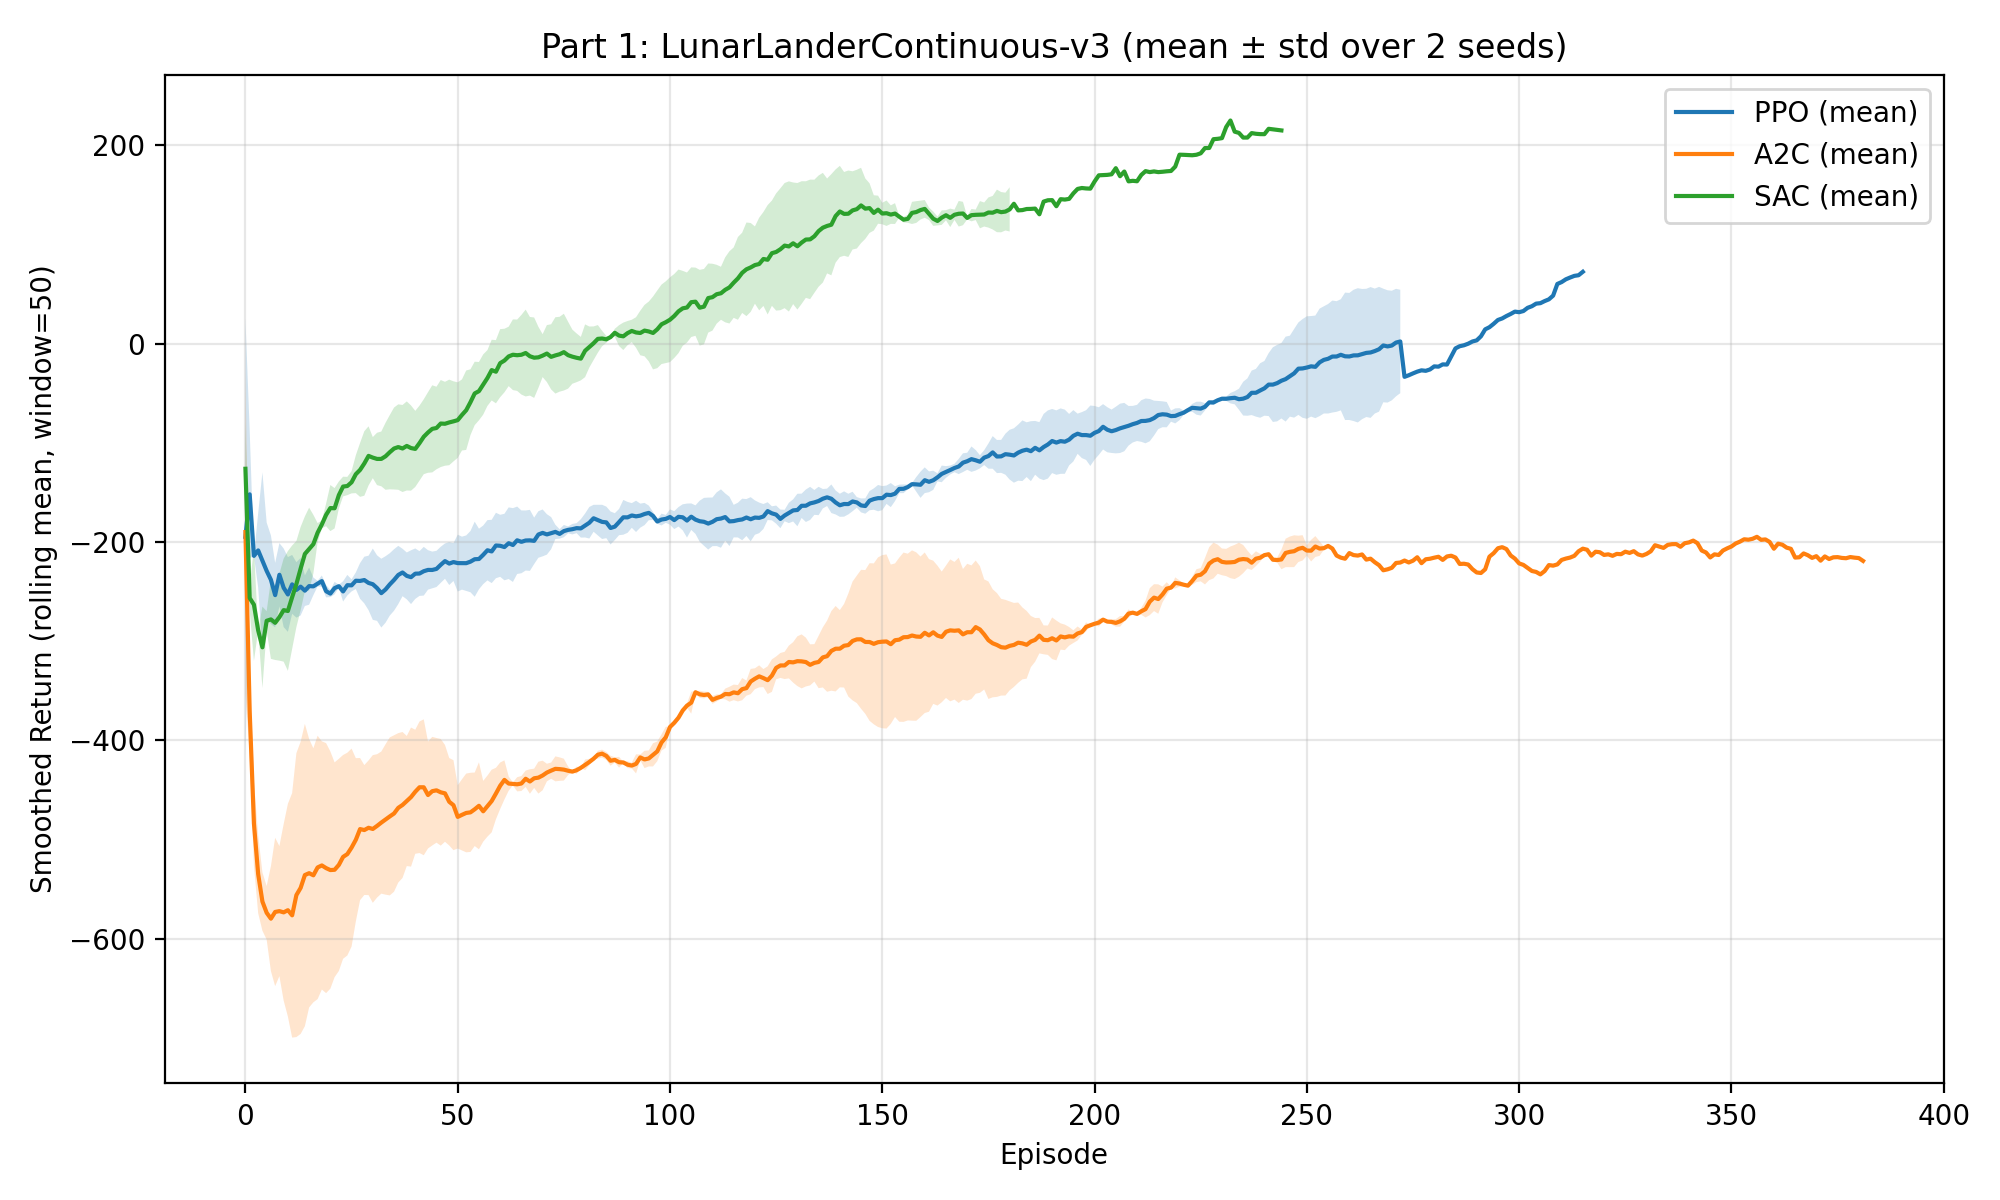
\includegraphics[width=0.85\textwidth]{../../neuro_v1/final_reports/part1/lunar_lander_comparison.png}
    \caption{Smoothed episodic return (rolling mean over $50$ episodes) for LunarLanderContinuous\allowbreak -v3. Solid lines denote the mean across seeds $\{0,1\}$; shaded regions denote $\pm 1$ standard deviation.}
\end{figure}

\subsection{Quantitative Summary}
For a fixed budget of $100{,}000$ steps and training seeds $\{0,1\}$, the last-$50$-episode mean return was summarized as mean $\pm$ standard deviation across seeds:
\begin{itemize}
    \item PPO: $55.76 \pm 23.60$.
    \item SAC: $167.31 \pm 67.45$.
    \item A2C: $-212.05 \pm 9.93$.
\end{itemize}
The number of completed episodes also differed substantially, reflecting differences in average episode length induced by policy quality under the same interaction budget. Across seeds, the mean episode counts were $294.5 \pm 30.4$ (PPO), $318.5 \pm 89.8$ (A2C), and $213.0 \pm 45.3$ (SAC).

\subsection{Sample Efficiency Proxy}
As a coarse proxy for sample efficiency at moderate performance, we measured the first episode index at which the smoothed return reached at least $80$. Under the fixed training horizon, SAC reached this level in both seeds (episode indices $114$ and $137$, mean $125.5$), while PPO and A2C did not reach this threshold within $100{,}000$ steps. This indicates that, under the present hyperparameterization and compute budget, replay-based off-policy learning combined with entropy-regularized exploration translated into faster attainment of moderate returns.

\subsection{Mechanistic Interpretation}
The observed trends can be explained by the structural properties of each algorithm.
\begin{itemize}
    \item \textbf{A2C underperformed due to unconstrained on-policy updates:} With short rollouts ($n_{\mathrm{steps}}=5$) and no trust-region constraint, the actor receives high-variance gradient estimates, while the critic is trained on short-horizon bootstrap targets. In a contact-rich physics domain, this can lead to rapid oscillations in policy parameters, producing consistently negative returns under the fixed budget.
    \item \textbf{PPO achieved stable improvement through clipped updates:} The clipping mechanism restricts the effective policy update when $r_t(\theta)$ deviates too far from $1$, reducing sensitivity to transient critic errors. This tends to yield smoother learning curves and fewer catastrophic collapses, particularly when reward shaping produces large magnitude changes early in training.
    \item \textbf{SAC exhibited strong performance but higher variance:} Off-policy learning with replay improves sample efficiency, but value overestimation, stochastic exploration induced by entropy maximization, and the non-stationarity of the replay distribution can cause episodic returns to vary widely at fixed training horizons. The high standard deviation is consistent with a mixture of successful landings and crash episodes under a still-exploring policy.
\end{itemize}

\subsection{Sample Efficiency and Stability}
Under an equal step budget, both PPO and SAC reached positive returns in the final training phase, whereas A2C did not. SAC can, in principle, be more sample-efficient due to replay, but the maximum-entropy objective can also sustain exploration longer, which may delay convergence to a highly deterministic landing strategy. PPO, while on-policy, trades sample efficiency for update stability, which was beneficial in this experiment.

\section{6.\ Critical Discussion}
The comparative study highlights a theory--practice alignment with important caveats.
\begin{itemize}
    \item \textbf{Why SAC can outperform on continuous control:} In continuous domains, the ability to reuse experience reduces the number of fresh environment interactions needed to refine a control policy. This is particularly advantageous when each episode contains long transients and costly failures.
    \item \textbf{Why PPO can be competitive despite being on-policy:} Stability mechanisms can dominate in moderately sized neural networks trained on non-linear physics. Clipped updates act as a regularizer against erroneous advantage estimates, often producing reliable improvement even when hyperparameters are not heavily tuned.
    \item \textbf{Sensitivity and statistical confidence:} The seed-to-seed variability observed for SAC was substantially larger than for PPO and A2C, suggesting sensitivity to stochastic exploration and critic bootstrapping effects under a short training horizon. Although the inclusion of multiple seeds improves statistical reporting, the small number of seeds limits confidence in fine-grained rankings; consequently, conclusions are presented at the level of qualitative trends rather than definitive performance claims.
\end{itemize}

\newpage
\chapter{Part 2: Custom Environment Design \& Training}

\section{7.\ Environment Design}
We developed a custom environment, \textbf{NeuroShot-v1}, modeling a single-shot interception problem: a stationary launcher must fire a projectile so that its ballistic trajectory intersects a moving target (a basket) whose motion combines linear drift and oscillation under an exogenous wind field. Each episode consists of exactly one decision followed by deterministic physics simulation, making the task a challenging instance of \emph{one-step planning with delayed consequence}. The environment was implemented with a lightweight 2D rendering and simulation stack based on Pygame~\cite{pygame}.

\subsection{Task Narrative and Decision-Critical Dynamics}
At the start of an episode, the basket is positioned at a random horizontal coordinate and moves leftward at a random speed while oscillating sinusoidally. The projectile experiences gravitational acceleration and a horizontal wind acceleration. The agent observes the current conditions and selects a launch force and angle. The reward depends only on the final miss distance at impact time, which forces the policy to learn \emph{anticipation}: good actions depend on a prediction of the basket position at a future time determined by the chosen launch parameters.

\subsection{Why NeuroShot-v1 is an Interesting RL Problem}
Although the episode contains a single action, the mapping $(s_0,a_0)\mapsto r_0$ is highly non-linear due to trigonometric coupling, the sinusoidal target trajectory, and the wind-induced quadratic term in horizontal displacement. The environment is also \emph{partially informative} rather than fully observable in the strict Markov sense because unmodeled latent factors (e.g., contact geometry tolerances) and normalization can obscure absolute scales; nevertheless, the provided observation contains sufficient information to learn a near-optimal policy.

\section{8.\ MDP Specification (Custom)}
The custom task is defined as an MDP $\mathcal{M}_{\mathrm{NS}}=(S,A,T,R,\gamma)$ with a single-step episode structure.

\subsection{State Space \texorpdfstring{$S$}{S}}
The observation is a normalized vector $s\in\mathbb{R}^7$ encoding target dynamics and projectile position:
\[
s=\left(\frac{x_b}{W},\ \frac{v_b}{20},\ \frac{w}{5},\ \frac{A}{50},\ \frac{f}{2},\ \frac{x_p}{W},\ \frac{y_p}{H}\right),
\]
where $W=800$ and $H=400$ are the world dimensions in pixels, $(x_b,v_b)$ are the basket position and horizontal speed, $w$ is the wind acceleration parameter, $(A,f)$ are oscillation amplitude and frequency, and $(x_p,y_p)$ is the projectile position. Initial conditions are randomized as:
\[
\begin{aligned}
x_b &\sim \mathrm{Unif}(400,700), & v_b &\sim \mathrm{Unif}(-10,-5),\\
w &\sim \mathrm{Unif}(-3,3), & A &\sim \mathrm{Unif}(20,50),\\
f &\sim \mathrm{Unif}(0.5,2.0).
\end{aligned}
\]

\subsection{Action Space \texorpdfstring{$A$}{A}}
The action is two-dimensional and continuous: $a=(a_0,a_1)\in[-1,1]^2$. It is mapped to physical launch parameters by affine transforms:
\[
V_0 = 30 + 40(a_0+1),\qquad \theta = \left(15^\circ + 35^\circ(a_1+1)\right)\cdot \frac{\pi}{180}.
\]
Thus $V_0\in[30,110]$ and $\theta\in[15^\circ,85^\circ]$.

\subsection{Transition Dynamics \texorpdfstring{$T$}{T}}
Given an action, the environment simulates projectile motion at time step $\Delta t=0.03$ with gravitational acceleration $g=9.8$ and horizontal wind acceleration $w$. Let the launch point be $(x_0,y_0)=(50,350)$ and define $v_x=V_0\cos\theta$ and $v_y=V_0\sin\theta$. The projectile trajectory is
\[
x_p(t)=x_0 + v_x t + \tfrac{1}{2} w t^2,\qquad
y_p(t)=y_0 - \left(v_y t - \tfrac{1}{2} g t^2\right),
\]
and the basket trajectory is
\[
x_b(t)=x_b(0)+v_b t + A\sin(ft).
\]
The simulation terminates when the projectile crosses the ground level, and the episode ends immediately afterward with $\mathrm{terminated}=\mathrm{True}$.

\subsection{Reward Design \texorpdfstring{$R$}{R}}
The reward is based on the miss distance between the projectile and the basket center at impact time. Let $t^\ast$ denote the simulated time at termination. The basket has width $60$, hence its center is at $x_b(t^\ast)+30$. Define the miss error
\[
e=\left|x_p(t^\ast)-\left(x_b(t^\ast)+30\right)\right|.
\]
The shaped reward is
\[
R(s,a)= -0.05\,e + 100\,\mathbb{I}[e<25],
\]
where $\mathbb{I}$ is the indicator function. This design is intentionally dense: the linear penalty supplies a gradient signal even under persistent misses, while the hit bonus creates a clear success criterion.

\subsection{Shaping Trade-offs}
The shaping term improves learning speed but can bias the policy toward minimizing horizontal error at the terminal height rather than maximizing robustness to variations in oscillation parameters. In particular, because the reward ignores vertical misalignment, an agent can receive high reward if it matches the target center in $x$ at impact time even if the trajectory would be physically implausible in a higher-fidelity setting. This is a deliberate simplification to focus learning on temporal prediction rather than collision geometry.

\section{9.\ Algorithm Selection}
We trained the final agent using \textbf{PPO} and additionally performed a preliminary algorithm screening on NeuroShot-v1 with \textbf{PPO}, \textbf{A2C}, and \textbf{DDPG}.

\subsection{Justification for PPO on NeuroShot-v1}
The custom task has continuous actions, shaped rewards, and potentially brittle training dynamics due to the single-step episode structure. PPO was selected because:
\begin{itemize}
    \item \textbf{Update robustness:} Clipped objectives reduce the probability of destructive updates when advantage estimates are noisy or when reward magnitudes change rapidly during early exploration.
    \item \textbf{Appropriate inductive bias:} A stochastic policy over continuous parameters can represent uncertainty in the required ``lead'' distance and can gradually sharpen as learning proceeds.
    \item \textbf{Implementation simplicity for rapid iteration:} The environment underwent multiple design fixes (time step, reward reference point). A stable on-policy baseline supports iterative development without heavy tuning of replay-buffer dynamics.
\end{itemize}

\begin{figure}[H]
    \centering
    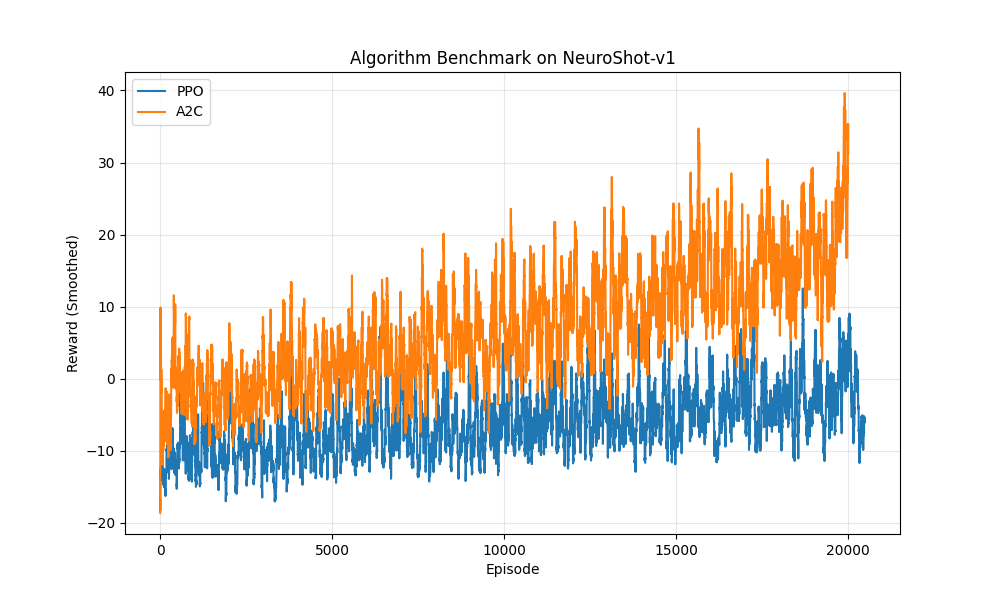
\includegraphics[width=0.85\textwidth]{../../neuro_v1/final_reports/benchmark/algo_comparison.png}
    \caption{Preliminary algorithm screening on NeuroShot-v1 comparing PPO, A2C, and DDPG (smoothed episodic rewards).}
\end{figure}

\section{10.\ Results and Evaluation (Part 2)}
\subsection{Training Setup and Reproducibility}
Training used a discount factor $\gamma=0.99$ and a total budget of $1{,}500{,}000$ environment steps with seed $42$. The PPO configuration was:
\[
\begin{aligned}
\alpha &= 10^{-4}, & n_{\mathrm{steps}} &= 2048, & \text{batch size} &= 64,\\
\lambda_{\mathrm{GAE}} &= 0.95, & \epsilon &= 0.2, & c_e &= 0,\\
c_v &= 0.5, & \|\nabla\|_{\max} &= 0.5.
\end{aligned}
\]
The learned policy and value functions were parameterized by two-hidden-layer multilayer perceptrons with widths $(64,64)$ and $\tanh$ activations, with input dimension $7$ matching the observation vector.

\subsection{Learning Curves and Stability}
Training diagnostics were logged at intervals of $100{,}000$ steps. For each checkpoint, the average episodic reward over a trailing window and a success-rate proxy were computed. Success was operationalized as $\mathbb{I}[G>50]$, where $G$ is the episodic return, aligning with the presence of the $+100$ hit bonus.

\begin{figure}[H]
    \centering
    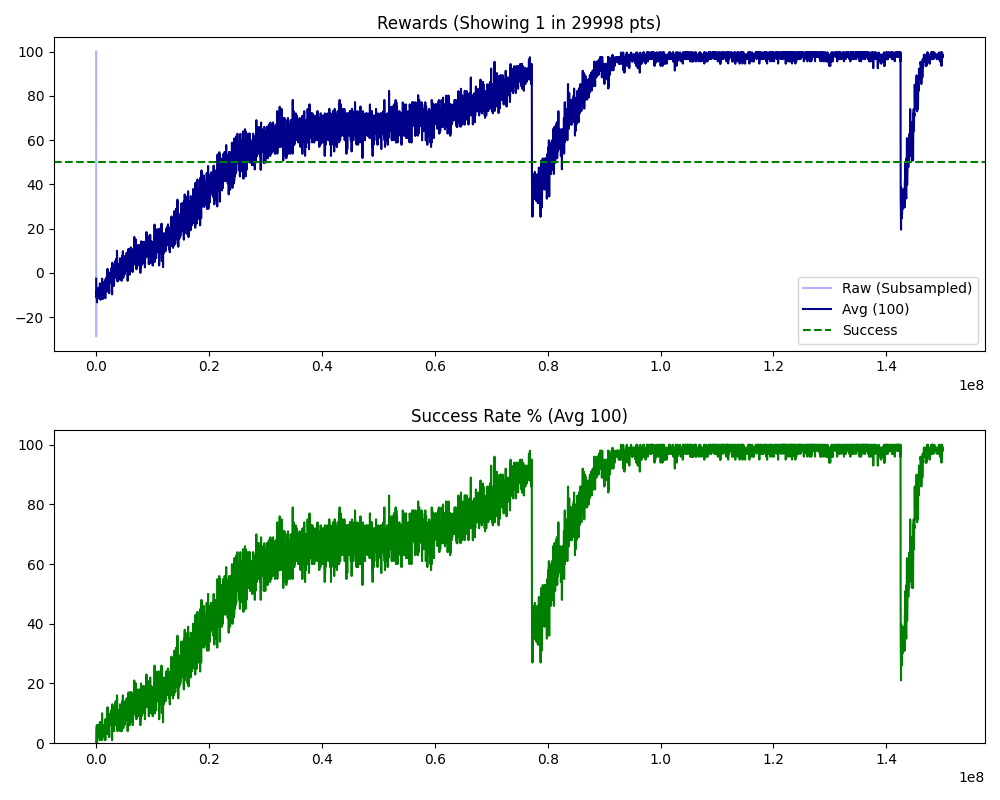
\includegraphics[width=0.85\textwidth]{../../neuro_v1/training_plots/progress_1500000.png}
    \caption{NeuroShot-v1 training diagnostics at $1{,}500{,}000$ steps: episodic rewards and success rate over training.}
\end{figure}

\subsection{Aggregated Metrics Across Runs}
The training log contains three appended runs. Aggregating by checkpoint step yields the mean and standard deviation across runs:
\begin{table}[H]
    \centering
    \caption{Aggregated performance across three training runs (mean $\pm$ standard deviation).}
    \begin{tabular}{ccc}
        \toprule
        \textbf{Steps} & \textbf{Reward} & \textbf{Success Rate} \\
        \midrule
        $100{,}000$ & $8.27 \pm 1.66$ & $0.13 \pm 0.02$ \\
        $500{,}000$ & $69.37 \pm 0.56$ & $0.70 \pm 0.01$ \\
        $800{,}000$ & $59.17 \pm 18.25$ & $0.60 \pm 0.18$ \\
        $1{,}000{,}000$ & $93.49 \pm 7.06$ & $0.94 \pm 0.07$ \\
        $1{,}100{,}000$ & $98.29 \pm 0.66$ & $0.99 \pm 0.01$ \\
        $1{,}500{,}000$ & $91.42 \pm 10.62$ & $0.92 \pm 0.10$ \\
        \bottomrule
    \end{tabular}
\end{table}
The pronounced variance around $800{,}000$--$900{,}000$ steps indicates sensitivity to the stochastic initial conditions (wind, oscillation) and to exploration noise. The later-stage stabilization around $1.0$--$1.1$ million steps suggests that the policy learned a robust mapping from observed target dynamics to a consistent lead-compensated launch configuration.

\subsection{Qualitative Policy Behavior}
The learned policy exhibits interpretable structure:
\begin{itemize}
    \item \textbf{Lead compensation:} As $v_b$ becomes more negative (faster leftward motion), the policy increases the implied horizontal travel time by adjusting $\theta$ upward (longer flight time) or increasing $V_0$ (greater range), effectively aiming ahead of the basket's instantaneous position.
    \item \textbf{Wind compensation:} Under $w<0$ (headwind), the policy increases $V_0$ and/or lowers $\theta$ to reduce time-of-flight and mitigate the quadratic wind term. Under $w>0$ (tailwind), it can reduce $V_0$ while maintaining accuracy.
    \item \textbf{Oscillation tracking:} Larger amplitude $A$ and higher frequency $f$ increase target unpredictability over the flight horizon. The policy tends to select shorter time-of-flight regimes (lower $\theta$, higher $V_0$) to reduce exposure to oscillatory phase uncertainty.
\end{itemize}

\subsection{Generalization Diagnostic: Accuracy Heatmap}
\begin{figure}[H]
    \centering
    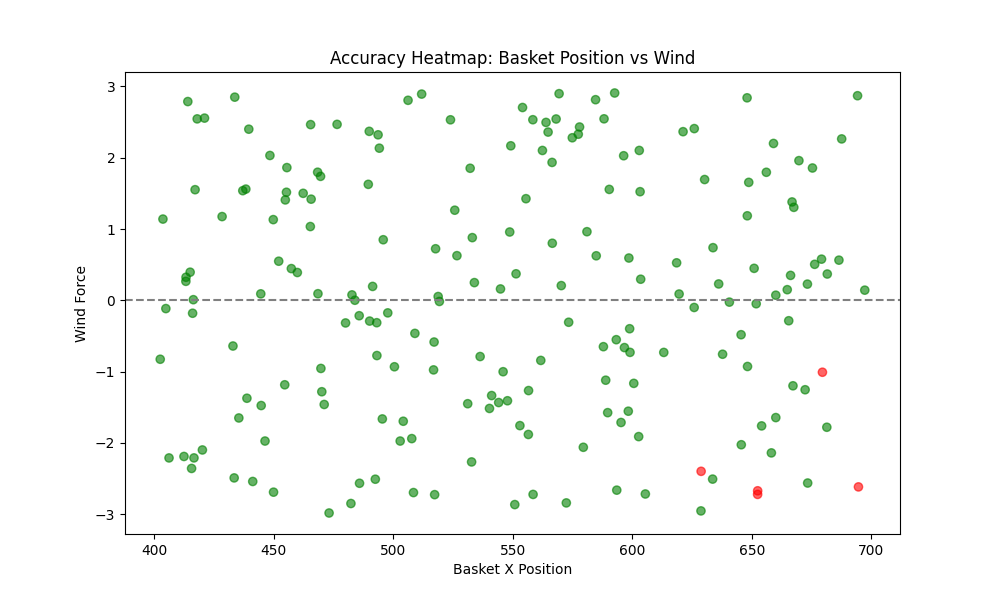
\includegraphics[width=0.85\textwidth]{../../neuro_v1/final_reports/accuracy_heatmap.png}
    \caption{Accuracy heatmap over test episodes: basket initial position vs.\ wind force. Green points denote hits ($e<25$), red denote misses.}
\end{figure}
The heatmap provides a qualitative generalization check over randomized initial conditions. Concentrations of misses at extreme wind magnitudes or at boundary basket positions would indicate extrapolation limits of the learned policy; conversely, a broad region of hits suggests robustness to joint variations in $x_b(0)$ and $w$.

\subsection{Failure Analysis}
Early training failures predominantly correspond to large miss errors in scenarios combining strong wind and high-frequency oscillation. From an RL perspective, these failures are consistent with \emph{credit assignment} difficulty: the reward is observed only after a variable-duration simulation, and naive exploration produces a near-uniform distribution over miss distances. The shaped penalty $-0.05e$ mitigates sparsity but does not eliminate the need to learn a temporally accurate internal predictor of $x_b(t^\ast)$.

\subsection{Final Policy Evaluation}
To complement training curves, we evaluated the final policy over 200 test episodes with randomized initial conditions. The evaluation yielded a mean episodic return of $71.50 \pm 45.08$ and a success rate of $72.5\%$, where success was defined as achieving episodic return $G>50$. The average miss error was $19.96$ pixels, consistent with a policy that frequently lands within the hit window but still exhibits failures under difficult wind--oscillation combinations.

\section{Additional Plots and Diagnostics}

\subsection{NeuroShot-v1 Evaluation Summary}
\begin{figure}[H]
    \centering
    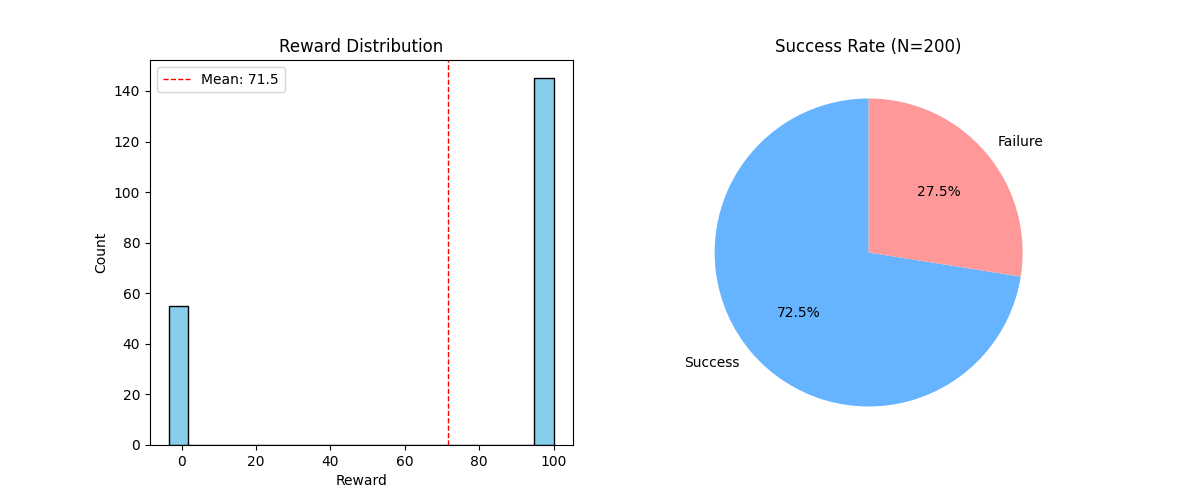
\includegraphics[width=0.95\textwidth]{../evaluation/eval_summary_NeuroShot-v1.png}
    \caption{Evaluation diagnostics for the trained NeuroShot-v1 policy over $200$ episodes: reward histogram and success rate summary.}
\end{figure}

\subsection{Benchmark Reproducibility Artifact}
For completeness, the benchmark aggregation across seeds used in Part 1 was exported as a structured summary containing the seeds, episode counts, and last-window statistics. This artifact supports reproducibility of reported mean and variance values and is stored alongside the Part 1 plot.

\subsection{Key Algorithmic Update Structure (Equation-Level)}
The following summarizes the training-update loops at the level of mathematical operations, complementing the main theoretical objectives in Part 1.
\begin{itemize}
    \item \textbf{PPO:} Collect a rollout of length $n_{\mathrm{steps}}$ under $\pi_{\theta_{\mathrm{old}}}$, compute generalized advantage estimates
    \[
    \hat{A}_t=\sum_{l=0}^{\infty}(\gamma\lambda)^l\delta_{t+l},\qquad \delta_t=r_t+\gamma V_\phi(s_{t+1})-V_\phi(s_t),
    \]
    form return targets $\hat{V}_t=\hat{A}_t+V_\phi(s_t)$, and optimize the composite objective $\mathcal{L}_{\mathrm{PPO}}(\theta,\phi)$ over multiple epochs using minibatches drawn from the rollout.
    \item \textbf{A2C:} Collect short rollouts of length $n$ (here $n=5$), compute $n$-step targets $\hat{G}_t^{(n)}$ and advantages $\hat{A}_t=\hat{G}_t^{(n)}-V_\phi(s_t)$, and apply a single joint gradient step minimizing $\mathcal{L}_{\mathrm{A2C}}(\theta,\phi)$ on the collected batch.
    \item \textbf{SAC:} Sample mini-batches from a replay buffer and update critics by minimizing a soft Bellman residual using the target
    \[
    y=r+\gamma\left(\min_{i\in\{1,2\}}Q_{\bar{\psi}_i}(s',a')-\alpha\log\pi_\theta(a'\mid s')\right),\qquad a'\sim \pi_\theta(\cdot\mid s'),
    \]
    then update the actor by minimizing $J_\pi(\theta)=\mathbb{E}[\alpha\log\pi_\theta(a\mid s)-Q_\psi(s,a)]$ and (optionally) update $\alpha$ to match a target entropy.
\end{itemize}

\subsection{Submission Notes}
The code repository link is submitted separately as per the project instructions. The custom environment NeuroShot-v1 was authored specifically for this project and is not a re-skin of an existing benchmark task.

\section{Conclusion}
This project studied deep reinforcement learning from both algorithmic and environment-design perspectives.
\begin{itemize}
    \item \textbf{Part 1:} Under a fixed interaction budget on LunarLanderContinuous-v3, PPO and SAC achieved positive final-phase returns, while A2C remained strongly negative. The results align with theory: PPO benefits from conservative updates, while SAC benefits from off-policy replay and entropy-regularized exploration, albeit with larger return variance.
    \item \textbf{Part 2:} NeuroShot-v1 demonstrates that deep RL can learn anticipatory ballistic interception in a non-linear, stochastic setting. PPO achieved high success rates under randomized wind and oscillatory target motion, and the learned policy exhibited coherent compensation behaviors.
\end{itemize}

\subsection{Limitations}
\begin{itemize}
    \item \textbf{Single-action episode structure:} Because each episode ends after one action, the problem resembles contextual optimization more than long-horizon control. Extending to multi-shot episodes would introduce richer temporal structure and more realistic planning.
    \item \textbf{Model simplifications:} The physics ignore air drag and basket geometry beyond a horizontal hit window. This limits ecological validity and may overestimate real-world transferability.
    \item \textbf{Statistical reporting:} While we report mean and variance across seeds for Part 1 and across multiple training logs for Part 2, the number of independent seeds for the LunarLander benchmark remains small, and additional multi-seed experiments would increase confidence in the observed trends.
\end{itemize}

\subsection{Future Extensions}
\begin{itemize}
    \item \textbf{Multi-step decision-making:} Allow the agent to adjust aim over time (e.g., moving the launcher or performing multiple shots) to increase horizon length and test long-term credit assignment.
    \item \textbf{Robustness and domain randomization:} Randomize gravity, wind statistics, and oscillation families, then evaluate out-of-distribution performance to quantify generalization and improve robustness.
\end{itemize}

\begin{thebibliography}{99}
\bibitem{schulman2017ppo}
J.~Schulman, F.~Wolski, P.~Dhariwal, A.~Radford, and O.~Klimov.
\newblock Proximal Policy Optimization Algorithms.
\newblock \emph{arXiv preprint arXiv:1707.06347}, 2017.

\bibitem{mnih2016a3c}
V.~Mnih, A.~P. Badia, M.~Mirza, A.~Graves, T.~Lillicrap, T.~Harley, D.~Silver, and K.~Kavukcuoglu.
\newblock Asynchronous Methods for Deep Reinforcement Learning.
\newblock In \emph{Proceedings of the 33rd International Conference on Machine Learning (ICML)}, 2016.

\bibitem{haarnoja2018sac}
T.~Haarnoja, A.~Zhou, P.~Abbeel, and S.~Levine.
\newblock Soft Actor-Critic: Off-Policy Maximum Entropy Deep Reinforcement Learning with a Stochastic Actor.
\newblock In \emph{Proceedings of the 35th International Conference on Machine Learning (ICML)}, 2018.

\bibitem{sutton2018rl}
R.~S. Sutton and A.~G. Barto.
\newblock \emph{Reinforcement Learning: An Introduction}.
\newblock MIT Press, 2nd edition, 2018.

\bibitem{gymnasium}
F.~F. contributors.
\newblock Gymnasium: A Standard Interface for Reinforcement Learning Environments.
\newblock \url{https://gymnasium.farama.org/}.

\bibitem{sb3}
A.~Raffin, A.~Hill, A.~Gleave, A.~Kanervisto, M.~Erin, and N.~Dormann.
\newblock Stable-Baselines3: Reliable Reinforcement Learning Implementations.
\newblock \url{https://github.com/DLR-RM/stable-baselines3}.

\bibitem{pytorch}
A.~Paszke et~al.
\newblock PyTorch: An Imperative Style, High-Performance Deep Learning Library.
\newblock In \emph{Advances in Neural Information Processing Systems (NeurIPS)}, 2019.

\bibitem{pygame}
Pygame contributors.
\newblock Pygame: Python Game Development.
\newblock \url{https://www.pygame.org/}.
\end{thebibliography}

\end{document}
